\chapter{Specyfikacja wewnętrzna}

% \chapter{[Właściwy dla kierunku - np.Specyfikacja wewnętrzna]}
% Jeśli to Specyfikacja wewnętrzna:
% \begin{itemize}
% \item przedstawienie idei
% \item architektura systemu
% \item opis struktur danych (i organizacji baz danych)
% \item komponenty, moduły, biblioteki, przegląd ważniejszych klas (jeśli występują)
% \item przegląd ważniejszych algorytmów (jeśli występują)
% \item szczegóły implementacji wybranych fragmentów, zastosowane wzorce projektowe
% \item diagramy UML
% \end{itemize}


% \begin{itemize}
% \item wymagania funkcjonalne i niefunkcjonalne
% \item przypadki użycia (diagramy UML) - dla prac, w których mają zastosowanie
% \item opis narzędzi, metod eksperymentalnych, metod modelowania itp.
% \item metodyka pracy nad projektowaniem i implementacją - dla prac, w których ma to zastosowanie
% \end{itemize}

\section{Klasa OpenLeap}

\subsection{Wykorzystanie innych klas}
\quad Klasa OpenLeap korzysta z różnych bibliotek. Natomiast nie dziedziczy ona żadnej klasy. Zostały jedynie wykorzystane wybrane metody tworzonych obiektów wewnątrz klasy. 

% \begin{figure}[H]
%     \begin{center}
%         \includegraphics[width=10cm]{example-image-a}
%         \caption{Relacja klas} 
%     \end{center}
% \end{figure}

\quad OpenLeap wykorzystuje metody klasy \textbf{mediapipe.solutions.hands.Hands} oraz \textbf{cv2.VideoCapture}. Pierwsza klasa pozwala na stworzenie obiektu, którego zadaniem jest rozpoznawanie dłoni na podstawie podawanego obrazu. Druga klasa tworzy obiekt, który pozwala na pobranie obrazu z kamery, określenie jego wielkości oraz sprawdzenia, czy kamera jest w ogóle dostępna. 

\newpage
\subsection{Budowa klasy}

\begin{wrapfigure}[16]{r}{0.5\textwidth}
    \begin{center}
        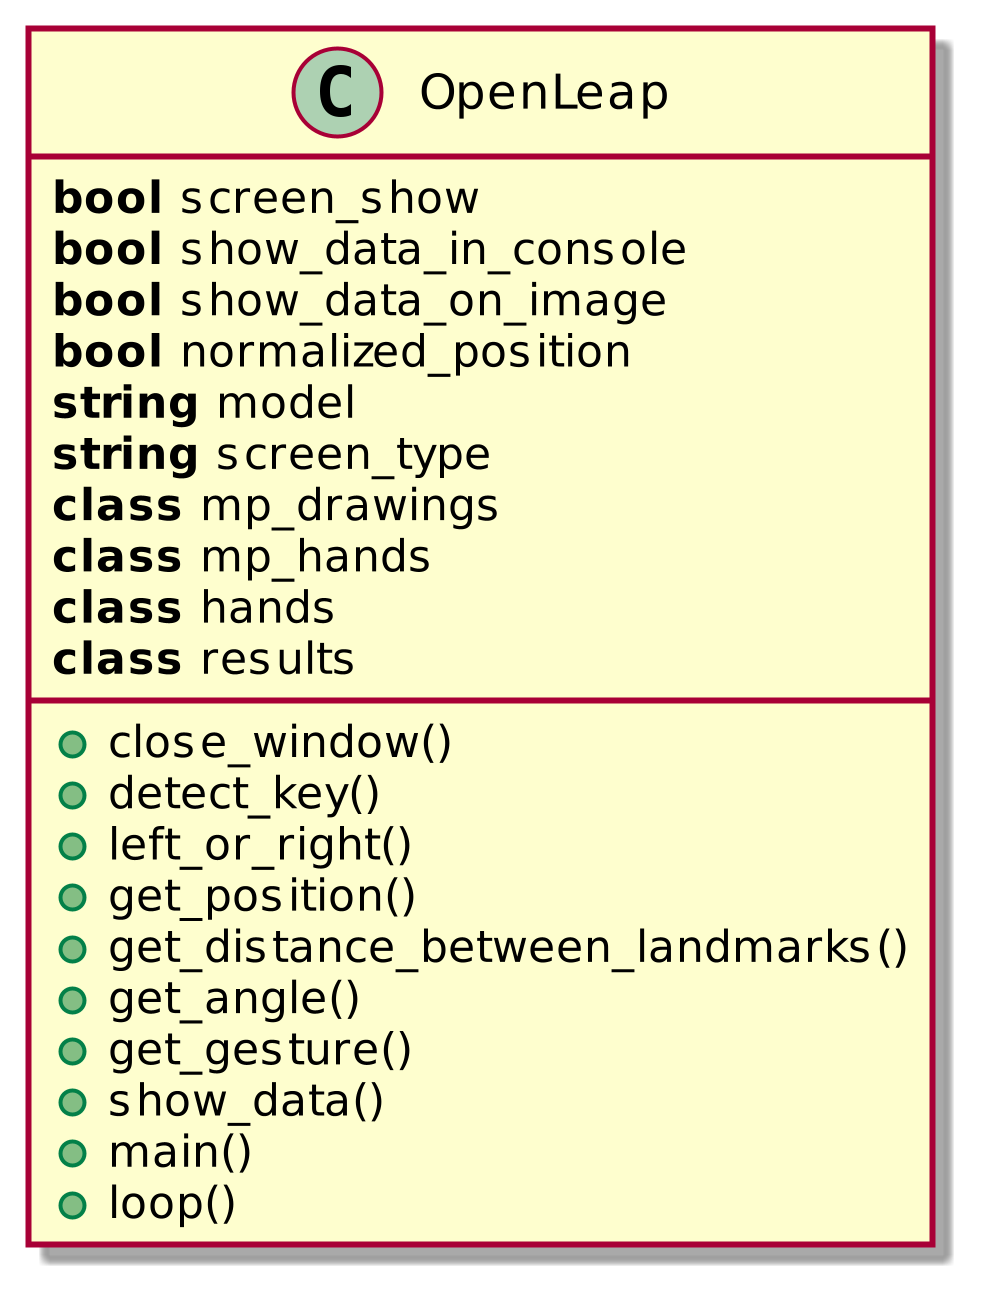
\includegraphics[width=0.48\textwidth]{../images/class.png}
        \end{center}
    \caption{Schemat klasy OpenLeap}
\end{wrapfigure}

\quad Klasa posiada atrybuty, których część jest parametrami, czyli dokładnie argumentami inicjalizatora klasy. Oprócz parametrów istnieją jeszcze zmienne oraz obiekty klas odpowiadające za rozpoznawanie dłoni, czy wykonanie operacji związanych z obliczeniem wartości zapisywanych w słowniku data, który też jest atrybutem klasy.

\quad Niektóre metody klasy mogą zostać wykonane automatycznie poprzez funkcje \textbf{main()} lub \textbf{loop()}. Natomiast można też wykonać potrzebne operacje bezpośrednio z wykorzystaniem wbudowanych metod, co może pomóc w optymalizacji programu. \newline\newline\newline\newline\newline\newline

% \begin{figure}[H]
%     \begin{center}
%         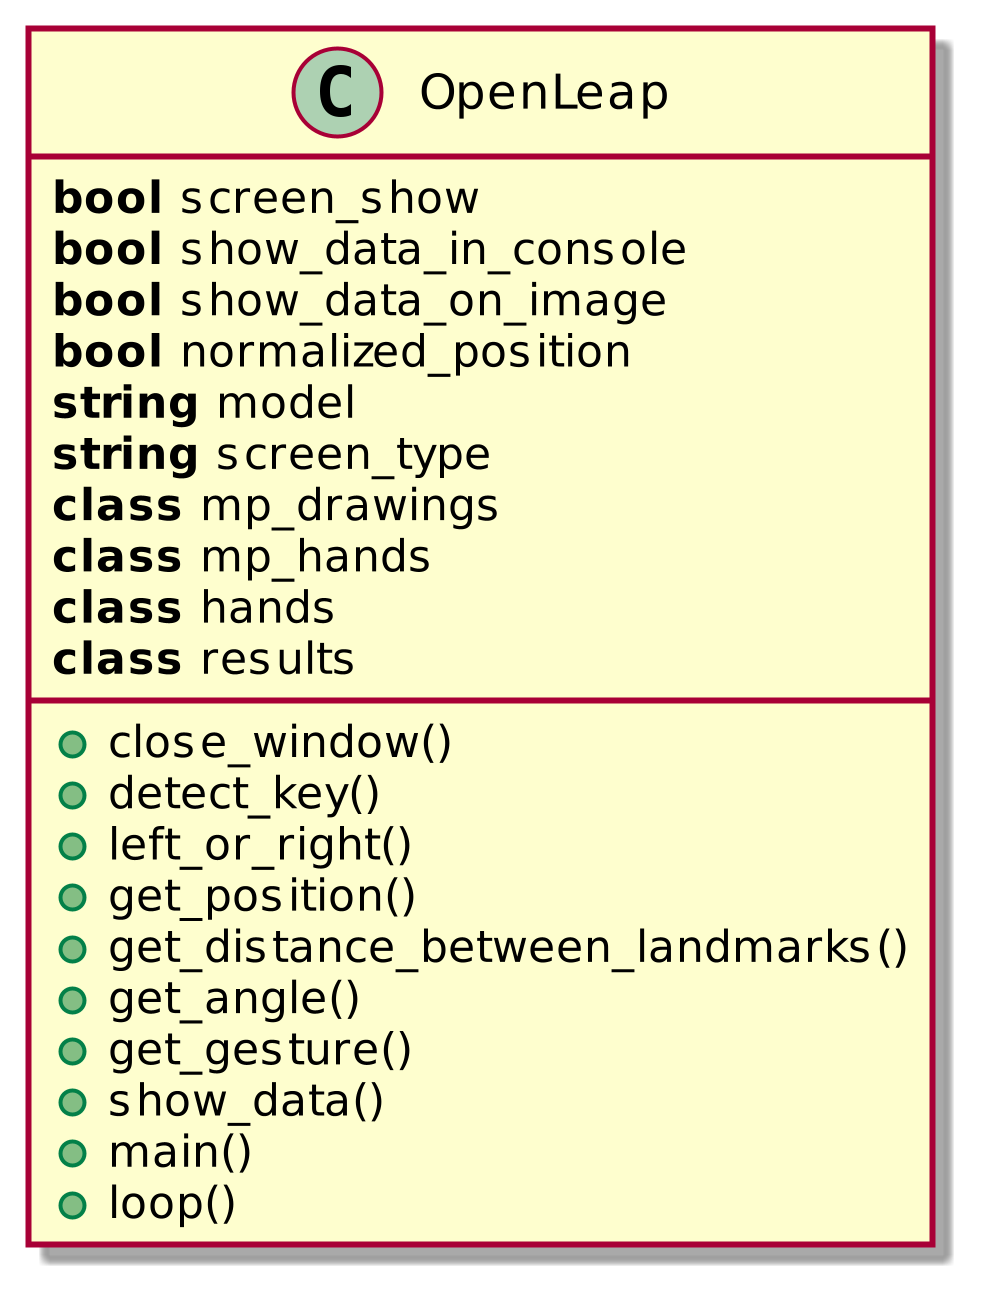
\includegraphics[width=7.5cm]{../images/class.png}
%         \caption{Schemat klasy OpenLeap} 
%     \end{center}
% \end{figure}


\subsection{Atrybuty klasy}

\quad Część atrybutów klasy została opisana w podrozdziale \textbf{\nameref{parametry}}, są to te elementy, które mogą zostać zdefiniowane przez użytkownika. Druga część atrybutów jest generowana automatycznie. 

\begin{enumerate}
    \item \textbf{mp\_drawings} --- Obiekt pobierany z biblioteki \textbf{MediaPipe} pozwalająca na rysowanie obrysu dłoni w oknie generowanym przez OpenCV.
    \item \textbf{mp\_hands} -- Obiekt przechowujący informacje, na przykład o indeksach opisujących poszczególne elementy charakterystyczne dłoni. 
    \item \textbf{hands} -- Model biblioteki MediaPipe rozpoznający dłonie. Inicjalizacja tego obiektu wymaga podania dwóch parametrów. 
    \begin{itemize}
        \item \textbf{min\_detection\_confidence} -- Minimalna wartość szacunkowa, dla której model określa czy została wykryta dłoń.
        \item \textbf{min\_tracking\_confidence} -- Minimalna wartość szacunkowa, pozwalająca określić dokładność śledzenia dłoni. 
    \end{itemize}
    \item \textbf{results} -- Obiekt przechowujący informacje o rozpoznanych dłoniach i ich elementach. 
    \item \textbf{data} -- Słownik, w którym są przechowywane informacje o obydwóch dłoniach. 
\end{enumerate}

\subsection{Metody klasy}

\quad W klasie zostały stworzone metody, które pozwalają na zbudowanie logiki programu. 

\begin{enumerate}
    \item \textbf{close\_window()} -- Zamknięcie wszystkich okien biblioteki OpenCV.
    \item \textbf{detect\_key()} -- Wykrycie kliknięcia wybranego przycisku podanego w argumencie.
    \item \textbf{left\_or\_right()} -- Metoda rozpoznająca lewą oraz prawą dłoń. Metoda za argumenty przyjmuje:
    \begin{itemize}
        \item \textbf{index} -- indeks badanej dłoni
        \item \textbf{mode} -- metoda określania typu dłoni 
        \begin{itemize}
            \item \textbf{\enquote{AI}} -- Wykorzystuje gotowy model MediaPipe. Niestety ten może nie zawsze działać poprawnie. 
            \item \textbf{\enquote{position}} -- Drugą metodą jest bazowanie na pozycji dłoni, dłoń po prawej stronie względem drugiej dłoni jest dłonią prawą i odwrotnie. Jeśli na ekranie widoczna jest jedna dłoń, wtedy funkcja jest wywoływana ponownie z argumentem \textbf{mode} ustawionym na \textbf{\enquote{AI}}.
        \end{itemize}
        \item \textbf{hand} -- Obiekt przechowujący współrzędne elementów charakterystycznych danej dłoni. 
    \end{itemize}
    \item \textbf{get\_position()} -- Funkcja zwraca pozycję elementu danej dłoni. 
    \begin{itemize}
        \item \textbf{index} -- indeks badanej dłoni
        \item \textbf{landmark\_idx} -- indeks elementu charakterystycznego, którego pozycję ma zwrócić funkcja
        \item \textbf{normalized} -- Parametr określający czy zwrócone współrzędne mają zostać znormalizowane.
    \end{itemize}
    \item \textbf{get\_distance\_between\_landmarks()} -- Metoda obliczająca odległość między dwoma wybranymi elementami charakterystycznymi.
    \begin{itemize}
        \item \textbf{index} -- Indeks dłoni, na której znajdują się mierzone elementy.
        \item \textbf{landmark\_1} -- indeks pierwszego elementu dłoni
        \item \textbf{landmark\_2} -- indeks drugiego elementu dłoni
        \item \textbf{normalized} -- Parametr określający czy odległość ma zostać znormalizowane.
    \end{itemize}
    \item \textbf{get\_angle()} -- Metod zwracająca kąt obrotu wybranego elementu charakterystycznego dłoni względem nadgarstka. 
    \begin{itemize}
        \item \textbf{index} -- indeks wybranej dłoni 
        \item \textbf{landmark\_idx} -- Indeks elementu względem, którego obliczany jest kąt.
        \item \textbf{mode}
        \begin{itemize}
            \item \textbf{half} -- kąt półpełny
            \item \textbf{full} -- kąt pełny
        \end{itemize}
        \item \textbf{unit}
        \begin{itemize}
            \item \textbf{radians} -- jednostka kąta w radianach
            \item \textbf{degrees} -- jednostka kąta w stopniach
        \end{itemize}
    \end{itemize}
    \item \textbf{get\_gesture()} -- Metoda określa gest wybranej dłoni. 
    \begin{itemize}
        \item \textbf{index} -- indeks wybranej dłoni
    \end{itemize}
    \newpage
    \item \textbf{show\_data()} -- Metoda wyświetlająca dane w oknie lub w konsoli w zależności od wybranej opcji. 
    \begin{itemize}
        \item \textbf{console} -- Flaga określająca czy dane mają zostać wypisane w konsoli.
        \item \textbf{on\_image} -- Flaga określająca czy dane mają zostać wypisane na ekranie. 
        \item \textbf{image} -- Wybrany obraz, na którym mają zostać wypisane dane.
    \end{itemize}
    \item \textbf{main()} -- Główna metoda, w której wykonywane są niezbędne obliczenia oraz funkcje. 
    \item \textbf{loop()} -- Metoda, w której wywoływana jest metoda \textbf{main()} w pętli. 
\end{enumerate}

\section{Struktury danych oraz pliki}

\quad Klasa zawiera w sobie parę struktur danych, które są kluczowe dla poprawnej pracy klasy oraz przechowywania informacji. Dobrze dobrane i zaprojektowane struktury danych pozwalają na pisanie programu, który jest przejrzysty i czytelny, na przykład poprzez wykorzystanie klasy \textbf{dataclass} zamiast tablicy czy słownika. 

\subsection{Struktura mp\_hands}

\quad Struktura mp\_hands jest enumeratorem. Przechowuje ona informacje o indeksach wszystkich elementów dłoni. Została ona stworzona po to, aby łatwiej było zapisywać program, który odczytuje informacje o danym elemencie. Ta struktura jest częścią biblioteki MediaPipe, więc jest już z góry zdefiniowana. 

\quad Pierwszym elementem określanym przez enumerator jest nadgarstek. Dalej znajduje się reszta elementów, oznaczająca resztę części palców i dłoni. Wszystkie elementy wraz z ich indeksami można zobaczyć na poniższej grafice \ref{img:hand_points}. To właśnie wyznaczenie pozycji tych elementów jest najważniejszą częścią, za która jest odpowiedzialna biblioteka MediaPipe i na której bazuje biblioteka OpenLeap. 

\begin{figure}[H]
    \begin{center}
        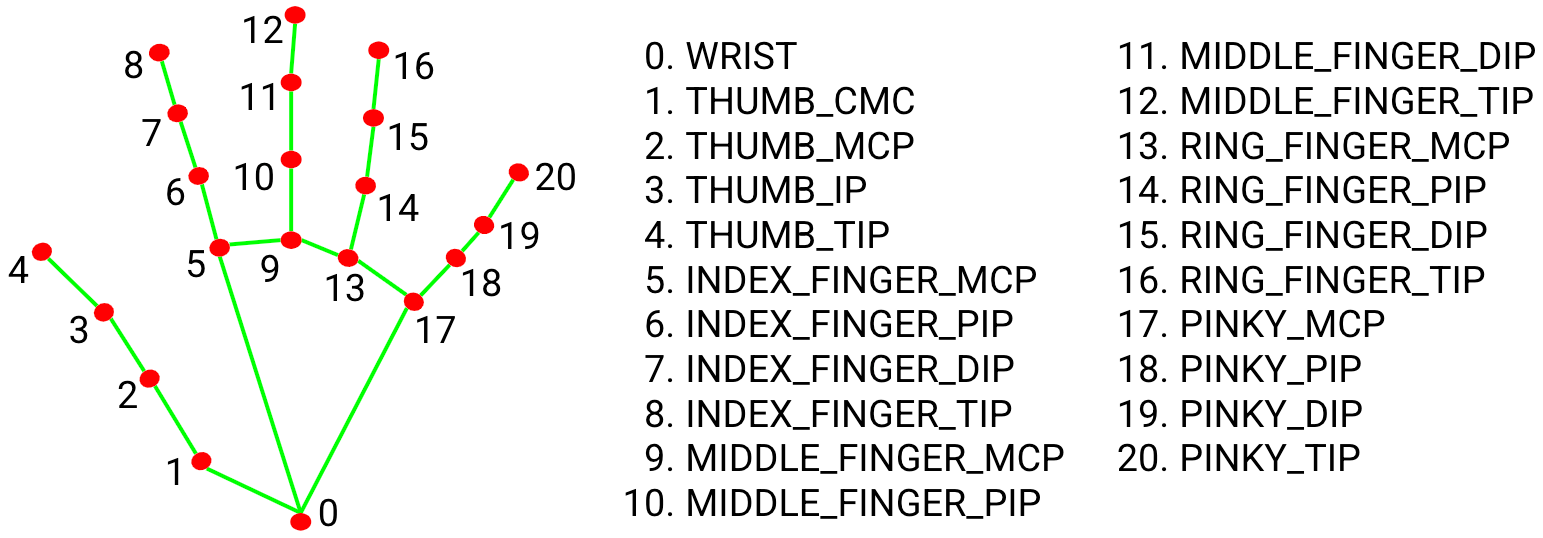
\includegraphics[width=12.8cm]{../images/hand_landmarks.png}
        \caption{Elementy charakterystyczne dłoni \cite{bib:mediapipe_img}}
        \label{img:hand_points}
    \end{center}
\end{figure}

\quad Przykład wykorzystania polega na odczytaniu współrzędnej X nadgarstka z listy o nazwie \textbf{landmark} będącej częścią obiektu \textbf{hand}. Jak można zobaczyć na przykładzie \ref{lst:enum}, wykorzystanie enumeratora pomaga w stworzeniu zapisu, który jest po prostu czytelny. \newline

\begin{lstlisting}[language=python, style=programming, caption={Przykładowe wykorzystanie \textbf{mp\_hands}},captionpos=b, label={lst:enum}]
    x = hand.landmark[self.mp_hands.HandLandmark.WRIST].x
\end{lstlisting}


\subsection{Struktura results}

\quad Struktura \textbf{results} jest obiektem, który przechowuje informacje zwrócone przez metodę \textbf{hands.process()}, czyli dokładanie dane, które są wygenerowane przy rozpoznawaniu dłoni. Obiekt składa się z dwóch list, które przechowują dane ogólne o dłoniach widocznych w obrazie oraz o szczególne dotyczące każdej dłoni z osobna. 

\begin{itemize}
    \item \textbf{multi\_hand\_landmarks} -- To pierwsza lista, która przechowuje dane o pozycjach wszystkich elementów danej dłoni. Odczyt danych wybranej dłoni wymaga podania jej indeksu. Indeksy punktów charakterystycznych można wybrać ze wcześniej wspomnianej struktury \textbf{mp\_hands}. \newpage
    
    \begin{lstlisting}[caption={Przykład korzystania z \textbf{multi\_hand\_landmarks}},captionpos=b,language=python, style=command]
    wrist_x = self.results.multi_hand_landmarks[index].landmark[self.mp_hands.HandLandmark.WRIST].x
    wrist_y = self.results.multi_hand_landmarks[index].landmark[self.mp_hands.HandLandmark.WRIST].y
    \end{lstlisting}

    \begin{lstlisting}[caption={Przykład elementu listy \textbf{multi\_hand\_landmarks}},captionpos=b,language=python, style=command]
    [landmark {
        x: 0.7409825921058655
        y: 0.6843034029006958
        z: 0.0
        }
        .
        .
        .
        landmark {
        x: 0.7874422073364258
        y: 0.26234549283981323
        z: -0.16528795659542084
        }
    ]
    \end{lstlisting}
    
      
    \item \textbf{multi\_handedness} -- Drugim typem jest lista przechowująca dane o wszystkich dłoniach widocznych na obrazie. Danymi są indeks, typ dłoni oraz punktacja określającą pewność poprawnego rozpoznania dłoni. Może posłużyć do sprawdzenia jaka jest liczba widocznych dłoni. \newline
    
    \begin{lstlisting}[caption={Przykład korzystania z \textbf{multi\_handedness}},captionpos=b,language=python, style=command]
    n_hands = len(self.results.multi_handedness)
    \end{lstlisting}

    \begin{lstlisting}[caption={Przykład elementu listy \textbf{multi\_handedness}},captionpos=b,language=python,style=command]
    [classification {
            index: 1
            score: 0.9482673406600952
            label: "Right"
        }
    ]
    \end{lstlisting}
\end{itemize}

\subsection{Dataclass}

\quad Klasa typu \textbf{Dataclass} pozwala na stworzenie struktury podobnej do \textbf{struct} istniejącej w języku programowania \textbf{C}. Taka klasa pozwala na stworzenie obiektu składającego się jedynie z atrybutów wymaganych do opisu danych generowanych podczas rozpoznawania dłoni. Dodatkowym atutem takiej klasy jest możliwość prostego odczytu zapisanych danych, korzystając z operatora kropki, a nie z operatorów wykorzystywanych w odczycie danych ze słownika lub listy.\newline 

\begin{lstlisting}[language=python, style=programming, captionpos=b, caption={Struktura Data}]
    @dataclass
    class Data:
        x : float = 0
        y : float = 0
        z : float = 0
        distance: float = 0.0
        angle: float = 0.0
        gesture: str = None
\end{lstlisting}

\quad W języku Python stworzenie klasy typu \textbf{dataclass} zaczyna się od zapisania dekoratora, który jest definiowany poprzez znak \textbf{@}. W tym wypadku nie jest wymagana funkcja inicjalizująca obiekt, czyli \textbf{\_\_init\_\_}. W definicji klasy zostały przypisane wartości początkowe tak jak w przykładzie powyżej. Dzięki czemu inicjalizacja nie wymaga podawania wartości początkowych, które i tak w chwili rozpoczęcia programu nie są potrzebne. 

\newpage
\subsection{Słownik}
\quad Instancja klasy \textbf{Data} jest przypisana dla każdej dłoni (lewej oraz prawej) poprzez wykorzystanie słownika. Klucze słownika to \enquote{right} oraz \enquote{left}.\newline 

\begin{lstlisting}[language=python, style=programming, captionpos=b, caption={Słownik przechowujący dane każdej z dłoni}]
    data = {'right':Data(), 'left':Data()}
\end{lstlisting}

\quad Taka konstrukcja pozwoli użytkownikowi w prosty i przejrzysty sposób na odnajdowanie potrzebnych wartości oraz informacji. Przykład odczytu informacji z tej struktury został już opisany w przykładzie \ref{lst:get_data1}

\subsection{Pickle}

\quad Modele rozpoznające gesty muszą zostać zapisane do pliku, tak aby można było z nich skorzystać po ich wygenerowaniu. W języku Python standardowym narzędziem wykorzystywanym do zapisu zmiennych lub obiektów służy plik typu \textbf{pickle}, który pozwala na zapis tych elementów w postaci binarnej. Pozwala to na ponownym odczyt obiektu po restarcie programu. W przypadku modelu rozpoznających gesty będzie można je zapisać właśnie z rozszerzeniem \textbf{.pickle}, a później odczytać je w chwili inicjalizacji obiektu klasy OpenLeap. 

\newpage
\section{Rozpoznawanie dłoni}

\quad Pierwszym elementem projektu jest rozpoznanie dłoni poprzez wyznaczenie pozycji elementów charakterystycznych. Pozycja każdego z tych elementów, jak już zostało to opisane, jest względna według lewego górnego rogu obrazu kamery. 

\begin{figure}[H]
    \begin{center}
        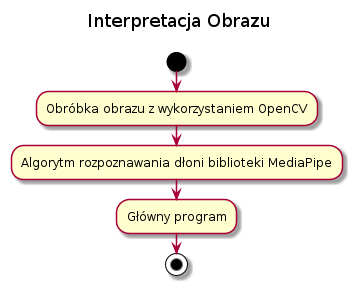
\includegraphics[width=10cm]{../images/image_processing.png}
        \caption{Przygotowanie obrazu}
    \end{center}
\end{figure}

\quad Obraz powinien zostać pozyskany z kamery oraz odpowiednio przetworzony przez funkcje biblioteki OpenCV. Kolejnym krokiem jest rozpoznanie elementów charakterystycznych dłoni przez model biblioteki MediaPipe. Na końcu powinna zostać wykonana główna część programu. Na przykład identyfikacja gestu czy obliczenia kąta obrotu dłoni. 

%%%%%%%%%%%%%%%%%%%%%%%%%%%%%%%%%%%%%%%%%%%%%%%%%%%%%%%%%%%%%%%%%%%%
%%%%%%%%%%%%%%%%%%%%%%%%%%%%%% OPEN CV %%%%%%%%%%%%%%%%%%%%%%%%%%%%%
%%%%%%%%%%%%%%%%%%%%%%%%%%%%%%%%%%%%%%%%%%%%%%%%%%%%%%%%%%%%%%%%%%%%
\subsection{OpenCV -- przygotowanie obrazu z kamery}

\quad Na początku należy zainicjalizować obiekt obsługujący kamerę. Argumentem jest identyfikator określający, która kamera podłączona do systemu ma zostać wykorzystana. W przypadku kiedy dostępna jest tylko jedna kamera, wystarczy wpisać wartość równą 0 tak jak poniżej.\newline

\begin{lstlisting}[language=python, style=programming, captionpos=b, caption={Wybór kamery}]
    self.cap = cv2 . VideoCapture (0)
\end{lstlisting}

\quad W metodzie \textbf{main()} w pierwszym kroku warunek określa czy zostało otwarte połączenie kamerą. Jeśli tak to należy pobrać z niej aktualną klatkę obrazu (\textbf{frame}). \newline

\begin{lstlisting}[language=python, style=programming, captionpos=b, caption={Przygotowanie funkcji głównej}]
    def main(self):
        """
        Main function that runs the core of the program. 
        """

        hand_type = None
        if self.cap.isOpened():
            ret, frame = self.cap.read()
\end{lstlisting}

\quad Model rozpoznający dłoń korzysta z przestrzeni barw RGB (red, green, blue), a nie BGR (blue, green, red), która jest standardem w OpenCV. Dlatego należy przekształcić obraz na przestrzeń RGB. Dodatkowo obraz powinien zostać obrócony horyzontalnie, tak aby stworzył lustrzane odbicie względem użytkownika ustawionego naprzeciwko kamery. Tak ustawiony obraz będzie lepiej sprawdzał się przy sterowaniu. \newline

\begin{lstlisting}[language=python, style=programming, captionpos=b, caption={Pierwsze przekształcenie}]
    #BGR to RGB
    image = cv2.cvtColor(frame, cv2.COLOR_BGR2RGB)

    #Flip horizontal
    image = cv2.flip(image, 1)
\end{lstlisting}


\quad Flaga \textbf{writeable} ustawiona na \textbf{False} pozwala na uzyskanie lepszej wydajności przy przetwarzaniu obrazu w ramach modelu rozpoznającego dłonie. Na co wskazuje dokumentacja biblioteki MediaPipe. Przy pomocy metody \textbf{process} będącej częścią obiektu \textbf{hands} zostają wygenerowane dane zapisywane do struktury \textbf{results}. Po tym etapie flaga \textbf{writeable} może zostać ustawiona z powrotem na wartość \textbf{True}. \newline 

\begin{lstlisting}[language=python, style=programming, captionpos=b, caption={Drugie przekształcenie}]
    #Set flag
    image.flags.writeable = False

    #Detections
    self.results = self.hands.process(image)
    # print(self.results.multi_hand_landmarks)

    #Set flag back to True
    image.flags.writeable = True
\end{lstlisting}

\quad Przestrzeń barw zostaje przywrócona do RGB, aby była mogła zostać poprawnie wyświetlona przez funkcję biblioteki OpenCV. \newline

\begin{lstlisting}[language=python, style=programming, captionpos=b, caption={Powrót do przestrzeni BGR}]
    #RGB to BGR
    image = cv2.cvtColor(image, cv2.COLOR_RGB2BGR)
\end{lstlisting}

%%%%%%%%%%%%%%%%%%%%%%%%%%%%%%%%%%%%%%%%%%%%%%%%%%%%%%%%%%%%%%%%%%%%
%%%%%%%%%%%%%%%%%%%%%%%%%%%% MEDIA PIPE %%%%%%%%%%%%%%%%%%%%%%%%%%%%
%%%%%%%%%%%%%%%%%%%%%%%%%%%%%%%%%%%%%%%%%%%%%%%%%%%%%%%%%%%%%%%%%%%%
\newpage

\section{Elementy charakterystyczne}

\quad Pozycje nadgarstka, paliczków oraz stawów dłoni zostaną wykorzystane do obliczenia kąta obrotu dłoni względem punktu 0, oraz do wytrenowania modeli uczenia maszynowego, których zadaniem będzie rozpoznawanie wybranych gestów. 

\subsection{Generowanie grafiki dłoni}

\quad Generowanie grafiki nałożonej na daną dłoń wykonuje się przy pomocy przygotowanej funkcji biblioteki MediaPipe, która współpracuje z OpenCV. Stworzenie oznaczeń polega na nałożeniu ich na obraz, który będzie wyświetlany w oknie. W tym wypadku jest to obraz o nazwie \textbf{background}, który przybiera formę czarnego tła lub obrazu z kamery w zależności od wybranej opcji. \newline

\begin{lstlisting}[language=python, style=programming, captionpos=b, caption={Obrys dłoni}]
    self.mp_drawing.draw_landmarks(background, 
            hand, 
            self.mp_hands.HAND_CONNECTIONS,
            self.mp_drawing.DrawingSpec(color=(75,50,200), 
                thickness=2, 
                circle_radius=2),
            self.mp_drawing.DrawingSpec(color=(225,180,10), 
                thickness=2, 
                circle_radius=2))
\end{lstlisting}

\quad Tworzone oznaczenia istnieją w dwóch formach. W postaci kropek nałożonych na nadgarstek i stawy oraz linii, które je łączą. 

\section{Pomiary oraz inne ważne elementy}
\quad Dane zapisywane w obiektach typu \textbf{Data} są generowane poprzez odpowiednie metody, które wykorzystują między innymi punkty charakterystyczne. 

\subsection{Rozpoznawanie typu dłoni}

\quad Rozpoznawanie typu dłoni wykonuje się na dwa różne sposoby. Pierwszym bazującym na metodach wykorzystujących uczenie maszynowe oraz drugim, który wykorzystuje względną pozycję dłoni względem siebie.  

\begin{itemize}
    \item \quad W pierwszym sposobie należy wyszukać w liście \textbf{multi\_handedness} słownika, który posiada w sobie indeks sprawdzanej dłoni i w tym samym słowniku sprawdzić, jaki jest jej typ. \newline

    \begin{lstlisting}[language=python, style=programming, captionpos=b, caption={Określenie typu dłoni -- Sposób nr 1}]
def left_or_right(self, index, mode='AI', hand=None):
    label = 'right'
        if mode == 'AI':
            
            for idx, classification in enumerate(self.results.multi_handedness):
                if classification.classification[0].index == index:

                    label = classification.classification[0].label.lower()

                    return label
    \end{lstlisting}

    \quad Jak się okazuje, nie jest to sposób, który daje zawsze poprawne rezultaty. Z tego powodu została stworzona alternatywny sposób wyznaczania typu dłoni. 

    \item \quad Poniższy sposób bazuje na założeniu, że lewa dłoń znajduje się na lewo od dłoni prawej, a prawa na prawo od lewej. Poprawność działania tego algorytmu wymaga jeszcze jednego założenia, że na ekranie powinny znajdować się dokładnie dwie dłonie, co nie zawsze może zostać spełnione. Można temu zapobiec poprzez wywołanie ponownie tej samej metody z wykorzystaniem pierwszego sposobu, kiedy na ekranie nie ma widocznych dwóch dłoni. \newline

    \begin{lstlisting}[language=python, style=programming, captionpos=b, caption={Określenie typu dłoni -- Sposób nr 2}]
    elif mode == 'position':
            coords = np.array((hand.landmark[self.mp_hands.HandLandmark.WRIST].x, hand.landmark[self.mp_hands.HandLandmark.WRIST].y))

            #Get x values from both hands and compare
            if len(self.results.multi_handedness) >= 2:
                for i in [0, 1]:
                    if index == i:
                        another_hand_x = self.results.multi_hand_landmarks[1-index].landmark[self.mp_hands.HandLandmark.WRIST].x
                        if coords[index] > another_hand_x:
                            label='right'
                        else:
                            label='left' 

                        return label
            else:
                return self.left_or_right(index, mode='AI', hand=hand)
    \end{lstlisting}
\end{itemize}

\subsection{Pozycja elementów}

\quad Metoda zwraca zwykłą lub znormalizowaną pozycję wybranego elementu dłoni. W dokumentacji można znaleźć informację, że normalizacja współrzędnej Z jest wykonywana względem szerokości obrazu tak jak współrzędnej X. Stąd też w przeliczeniu wartości znormalizowanych na zwykłe należy przemnożyć współrzędną Z przez szerokość obrazu tak jak współrzędną X. \newline

\begin{lstlisting}[language=python, style=programming, captionpos=b, caption={Pobranie pozycji}]
def get_position(self, index=0, landmark_idx=1, normalized=False):
    x = self.results.multi_hand_landmarks[index].landmark[landmark_idx].x
    y = self.results.multi_hand_landmarks[index].landmark[landmark_idx].y
    z = self.results.multi_hand_landmarks[index].landmark[landmark_idx].y

    if normalized:
        #Choose proper index instead of fixed one (idx=0)
        return x, y, z
    else:
        x = int(x*self.WIDTH)
        y = int(y*self.HEIGHT)
        z = int(z*self.WIDTH)
    return x, y, z
\end{lstlisting}

\subsection{Odległość między punktami}

\quad Odległość jest obliczana ze standardowego wzoru na odległość między dwoma punktami w wybranym układzie współrzędnych. 

\begin{equation}
    d = \sqrt{(x_1-x_2)^2 + (y_1-y_2)^2}
\end{equation}\newline
\quad Użytkownik ma możliwość wyboru czy wartość ma być liczona za pomocą zmiennych znormalizowanych, czy nie.  \newline

\begin{lstlisting}[language=python, style=programming, captionpos=b, caption={Obliczenie pozycji punktu charakterystycznego}]
def get_distance_bettween_landmarks(self, index, landmark_1, landmark_2, normalized=True):
    if normalized:
            x1, y1, z1 = self.get_position(index, landmark_1, normalized=True)
            x2, y2, z2 = self.get_position(index, landmark_2, normalized=True)
        else:
            x1, y1, z1 = self.get_position(index, landmark_1)
            x2, y2, z2 = self.get_position(index, landmark_2)

        distance = math.sqrt(((x1-x2)**2 + (y1-y2)**2))

        return distance
\end{lstlisting}

\subsection{Obrót dłoni}

\quad Obrót dłoni jest obliczany jako kąt obrotu ramienia, którego początek znajduje się w punkcie nadgarstka, a drugi koniec jest wybranym dowolnym punktem dłoni. Wykorzystana jest do tego funkcja \textbf{atan2()}, która za argumenty bierze współrzędne końca ramienia w układzie współrzędnych, którego środkiem jest nadgarstek. Dodatkowe argumenty funkcji \textbf{get\_angle()} określają zakres kąta oraz jego jednostkę. \newline

\begin{lstlisting}[language=python, style=programming, captionpos=b, caption={Obliczenie odległości między wybrany punktami}]
def get_angle(self, index, landmark_idx, mode='half', unit='radians'):
    angle=0

    wrist_x = self.results.multi_hand_landmarks[index].landmark[self.mp_hands.HandLandmark.WRIST].x
    wrist_y = self.results.multi_hand_landmarks[index].landmark[self.mp_hands.HandLandmark.WRIST].y

    landmark_x = self.results.multi_hand_landmarks[index].landmark[landmark_idx].x
    landmark_y = self.results.multi_hand_landmarks[index].landmark[landmark_idx].y

    realitive_x = landmark_x - wrist_x
    realitive_y = landmark_y - wrist_y

    angle = math.atan2(realitive_y, realitive_x)

    if mode=='half' and angle>0: angle=0

    if unit=='degree':
        angle = 180*abs(angle)/math.pi

    return angle

\end{lstlisting}

%%%%%%%%%%%%%%%%%%%%%%%%%%%%%%%%%%%%%%%%%%%%%%%%%%%%%%%%%%%%%%%%%%%%
%%%%%%%%%%%%%%%%%%%%%%%%%%% SciKit Learn %%%%%%%%%%%%%%%%%%%%%%%%%%%
%%%%%%%%%%%%%%%%%%%%%%%%%%%%%%%%%%%%%%%%%%%%%%%%%%%%%%%%%%%%%%%%%%%%

\section{Rozpoznawanie gestów}

\quad Modele pozwalają na rozpoznanie gestów na podstawie pozycji elementów dłoni. Aby było to możliwe, należy wytrenować modele na podstawie odpowiednio przygotowanych danych, czyli takich, które zależą jedynie od ułożenia dłoni. Należy również skorzystać z wcześniej opisanego pliku \textbf{pickle} tak, żeby model mógł zostać wczytany ponownie do programu. 
 
\subsection{Mechanizm załadowania modelu}

\quad Argumentem inicjalizatora klasy jest między innymi typ modelu rozpoznającego gesty lub ścieżka do tego pliku. Po ustaleniu odpowiedniej ścieżki należy wczytać plik jako plik binarny.  \newline 

\begin{lstlisting}[language=python, style=programming, captionpos=b, caption={Wczytanie modelu}]
with open(data_path, 'rb') as f:
    self.gesture_model = pickle.load(f)
\end{lstlisting}

\subsection{Wykorzystanie modelu}

\quad Do rozpoznania gestu została przygotowana funkcja, która zwraca nazwę rozpoznanego gestu. W poniższym przykładzie znajduje się jedynie linia o numerze 9, która wykorzystuje sam model. Metoda przeprowadza jeszcze odpowiednie przekształcenia danych, które zostaną opisane w podsekcji opisującej proces uczenia algorytmów. \newline

\begin{lstlisting}[language=python, style=programming, captionpos=b, caption={Funkcja zwracająca rozpoznany gest}]
def get_gesture(self, index):

    .
    .
    .

    with warnings.catch_warnings():
        warnings.filterwarnings("ignore")
        gesture_class = self.gesture_model.predict(x)[0]

    return gesture_class
\end{lstlisting}


\newpage
\section{Przygotowanie modeli uczenia maszynowego}

% \subsection{Przygotowanie modeli uczenia maszynowego}
\quad Zadaniem instrukcji uczącej będzie stworzenie modeli matematycznych przy pomocy algorytmów uczenia maszynowego, których celem jest rozpoznawanie gestów dłoni. Proces tworzenie takiego modelu można podzielić na trzy kroki przedstawione na schemacie \ref{img:full_algorithm}. 

\begin{figure}[H]
    \begin{center}
        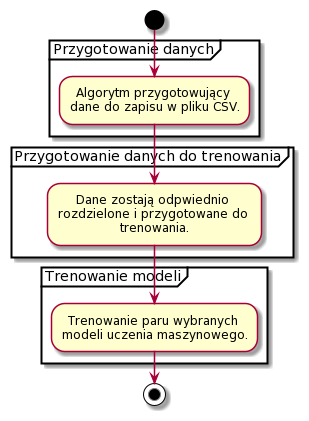
\includegraphics[width=8cm]{../images/full_algorithm.png}
        \caption{Ogólny algorytm przygotowania modeli uczenia maszynowego}
        \label{img:full_algorithm}
    \end{center}
\end{figure}

\quad Całość programu została napisana osobno w notatniku Jupyter. Pozwala to na wykonanie pewnych części programu osobno, niezależnie od reszty programu. W praktyce każdy blok opisany w powyższym schemacie UML ma swoje odwzorowanie w notatniku. Na przykład, część zapisująca współrzędne do pliku będzie wykonywana tyle razy, ile jest gestów do wytrenowania, co definiuje osoba trenująca w czasie działania programu. 

\quad Opisywany program może również pełnić funkcję instrukcji, o czym był mowa w podsekcji \ref{ext:new_model}.

\subsection{Zebranie danych}

\begin{wrapfigure}[22]{r}{0.5\textwidth}
    \begin{center}
        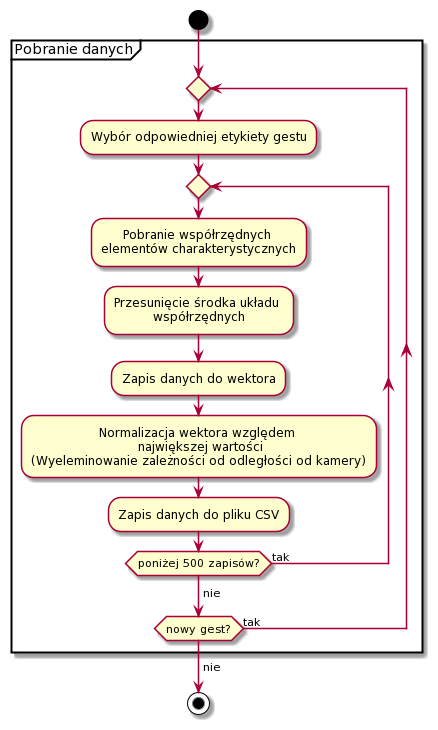
\includegraphics[width=9cm]{../images/get_data.png}
        \caption{Algorytm zbierania danych}
    \end{center}
\end{wrapfigure}

\quad Algorytm rozpoznający gesty powinien zostać wytrenowany na podstawie zbiorów współrzędnych punktów charakterystycznych i przypisanych do nich nazw gestów. Za nim to jednak nastąpi, należy zauważyć parę trudności z tym związanych. Podstawowym problemem jest fakt, że pozycje elementów charakterystycznych są opisane względem układu współrzędnych (można go uznać za układ bezwzględny), którego środek znajduje się w lewym górnym rogu obrazu pobranego z kamery. Wynika, więc z tego, że skorzystanie z tych współrzędnych jako danych uczących, skutkowałoby tym, że model klasyfikowałby gest również na podstawie jego pozycji na obrazie. W takim wypadku należy przeprowadzić transformację, tutaj akurat przesunięcie układu współrzędnych do pozycji nadgarstka (układ względny). \newpage

\quad Współrzędne w układzie bezwzględnym opisujące pozycje punktów można zapisać w poniższej macierzy. Liczby przy symbolach są równoważne z indeksami tablicy opisującej punkty, rys. \ref{img:hand_points}.

\begin{figure}[H]
    \begin{equation}
        M_G = 
        \begin{bmatrix}
        x_0 & y_0 & z_0 \\
        x_1 & y_1 & z_1 \\
            & \vdots &     \\
        x_{21} & y_{21} & z_{21}
        \end{bmatrix}
    \end{equation}    
    \caption{Pełna postać macierzy}
\end{figure}

\quad Przesunięcie układu współrzędnych można opisać poprzez macierz transformacji, gdzie wartości ${x_0, y_0, z_0}$ to współrzędne nadgarstka w bezwzględnym układzie współrzędnych.  

\begin{figure}[H]
    \begin{equation}
        M_p = 
        \begin{bmatrix}
            1 & 0 & 0 & -x_0 \\
            0 & 1 & 0 & -y_0 \\
            0 & 0 & 1 & -z_0 \\
            0 & 0 & 0 & 1
        \end{bmatrix}
    \end{equation}
    \caption{Macierz transformacji ogólna}
\end{figure}


\quad Tak naprawdę, przesunięcie układu współrzędnych wzdłuż osi Z nie będzie miało miejsca. Wartości współrzędnej Z wszystkich elementów są obliczane względem pozycji nadgarstka, co oznacza, że współrzędna Z nadgarstka wynosi zawsze 0. W takim wypadku można ją usunąć z macierzy przesunięcia. Ostatecznie macierz ma postać:  

\begin{figure}[H]
    \begin{equation}
        M_p = 
        \begin{bmatrix}
        1 & 0 & 0 & -x_0 \\
        0 & 1 & 0 & -y_0 \\
        0 & 0 & 1 & 0 \\
        0 & 0 & 0 & 1
        \end{bmatrix}
    \end{equation}
    \caption{Macierz transformacji szczególna}
\end{figure}

\quad Po przekształceniu macierzy współrzędne punktów są następującej postaci. Jak można zauważyć, współrzędne nadgarstka zostały kompletnie pominięte. Po operacji przesunięcia ich wartości zostały wyzerowane, więc nie zostały wpisane ponownie do macierzy. 

\begin{figure}[H]
    \begin{equation}
        M_G = 
        \begin{bmatrix}
        x_1' & y_1' & z_1' \\
        x_2' & y_2' & z_2' \\
            & \vdots &     \\
        x_{21}' & y_{21}' & z_{21}'
        \end{bmatrix}
    \end{equation}    
    \caption{Pełna postać macierzy}
\end{figure}

\quad Aby dane mogły zostać poprawnie zinterpretowane przez algorytmy uczenia maszynowego, muszą one zostać przedstawione w postaci jednowymiarowej. Macierz zostaje przekształcona do postaci następującego wektora. 

\begin{figure}[H]
    \begin{equation}
        A_f=
        \begin{bmatrix}
            x_1' & y_1' & z_1' & x_2' & y_2' & z_2' & \cdots & x_{21}' & y_{21}' & z_{21}'
        \end{bmatrix}
    \end{equation}  
    \caption{Wektor danych}
\end{figure}

\quad Kolejnym krokiem jest uniezależnienie pozycji elementów od odległości dłoni od kamery. Rozwiązaniem jest normalizacja wektora danych względem największej bezwzględnej wartości. 

\begin{figure}[H]
\begin{equation}
    A_n=\dfrac{A_f}{max(abs(A_f))}
\end{equation}
\caption{Normalizacja wektora danych}
\end{figure}

\quad Każdy nowy wektor zostaje zapisany do pliku CSV z odpowiednią etykietą. Tak zebrane i przetworzone dane posłużą do wytrenowania algorytmów uczenia maszynowego.

\newpage
\subsection{Praktyczne wykorzystanie}

\quad Do programu zostają pobrane pozycje wszystkich elementów. Później zostaje stworzona pusta tablica o wymiarach 20x3, która zostaje zapisana współrzędnymi po operacji przesunięcia. \newline

\begin{lstlisting}[language=python, style=programming, captionpos=b, caption={Przygotowanie wektora danych}]
    hand_landmarks = results.multi_hand_landmarks[0].landmark
    wrist = hand_landmarks[0]

    hand_landmarks_row = np.zeros((20,3))
    for i in range(1, len(hand_landmarks)):
        hand_landmarks_row[i-1]=[hand_landmarks[i].x-wrist.x, 
                                hand_landmarks[i].y-wrist.y, 
                                hand_landmarks[i].z-wrist.z]
\end{lstlisting}

\quad Kolejnym krokiem jest przekształcenie macierzy na wektor (funkcja \textbf{flatten()}) oraz znormalizowanie tego wektora. Ostatecznie wektor zostaje zapisany do pliku CSV wraz z odpowiednią etykietą. \newline

\begin{lstlisting}[language=python, style=programming, captionpos=b, caption={Przygotowane wektora danych}]
    hand_landmarks_row = hand_landmarks_row.flatten()
    hand_landmarks_row = list(hand_landmarks_row/np.max(np.absolute(hand_landmarks_row)))
    
    hand_landmarks_row.insert(0, class_name)
    
    with open(FILE_NAME, mode='a', newline='') as f:
        csv_writer = csv.writer(f, 
                                delimiter=',', 
                                quotechar='"', 
                                quoting=csv.QUOTE_MINIMAL)

        csv_writer.writerow(hand_landmarks_row)
\end{lstlisting}

\subsection{Budowa pliku CSV}
\quad Dane zapisane w pliku CSV opisują przykładowe współrzędne wszystkich elementów dłoni wraz z przypisaną etykietą oznaczającą gest. Poniżej zostały przedstawione przykładowe dane trenujące dla modelu podstawowego, czyli rozpoznającego otwartą i zamkniętą dłoń. \newline

\textbf{Początek}\newline

\begin{table}[H]
\centering
\csvautotabular{head.csv} 
\caption{Początek pliku}
\end{table}

\textbf{Koniec}\newline

\begin{table}[H]
\centering
\csvautotabular{tail.csv} 
\caption{Koniec pliku}
\end{table}

\newpage
\subsection{Metody klasyfikacji -- uczenie maszynowe}

\quad Przygotowane dane zostają odczytane z pliku CSV. W pierwszym kroku należy rozdzielić je na dwie części: współrzędne (dane wejściowe) oraz etykiety (dane wyjściowe). W drugim kroku należy te dwie grupy podzielić na grupę trenującą i grupę testową. Zadaniem grupy testowej będzie trenowanie wybranych modeli, a grupy testowej przetestowanie ich dokładności. 

\quad Poniższy schemat przedstawia działanie części wykorzystującej wiele algorytmów uczenia maszynowego do wyznaczenia modelu o największej poprawności działania. 

\begin{figure}[H]
    \begin{center}
        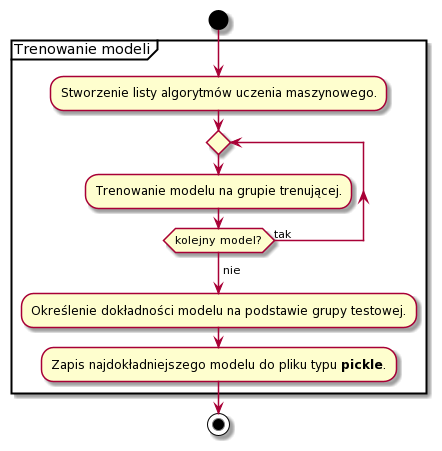
\includegraphics[width=11cm]{../images/train_models.png}
        \caption{Algorytm trenowania wielu modeli}
    \end{center}
\end{figure}

\quad W celu wybrania najlepszej metody klasyfikacji zostanie wybranych kilka algorytmów. Każdy z nich stworzy swój model, a ostatecznie zostanie sprawdzona ich poprawności z wykorzystaniem grupy testowej. Model z najlepszym wynikiem zostanie zapisany do pliku typu \textbf{pickle}.

\subsection{Wybrane algorytmy klasyfikujące}

\quad Do wytrenowania modeli uczenia maszynowego z biblioteki SciKit-Learn \cite{bib:ml} zostały wybrane następujące algorytmy:

\begin{itemize}
    \item Logistic Regression %(\enquote{Regresja Logistyczna})
    \item Nearest Centroid 
    \item Decision Tree Classifier
    \item Ridge Classifier 
    \item Random Forest Classifier 
    \item SGD Classifier
    \item Gradient Boosting Classifier
    \item MPL Classifier
\end{itemize}

\quad Algorytmy można zapisać w słowniku, który później pozwoli na wykorzystanie ich w pętli. \newline

\begin{lstlisting}[language=python, style=programming, captionpos=b, caption={Funkcja zwracająca rozpoznany gest}]
pipelines = {
'lr':make_pipeline(StandardScaler(),LogisticRegression()),
'nc':make_pipeline(StandardScaler(),NearestCentroid()),
'dt':make_pipeline(StandardScaler(),DecisionTreeClassifier()),
'rd':make_pipeline(StandardScaler(),RidgeClassifier()),
'rf':make_pipeline(StandardScaler(),RandomForestClassifier()),
'gd':make_pipeline(StandardScaler(),SGDClassifier()),
'gb':make_pipeline(StandardScaler(),GradientBoostingClassifier()),
'nn':make_pipeline(StandardScaler(),MLPClassifier()),
}
\end{lstlisting}

\quad \textbf{Pipline} pozwala na zautomatyzowanie pewnych procesów związanych z uczeniem. Tutaj, na przykład zostaje wykorzystane funkcja \textbf{StandardScaler()}, która odpowiednio standaryzuje dane wejściowe. 

\begin{lstlisting}[language=python, style=programming, captionpos=b, caption={Trenowanie modeli}]
models = {}
for algorithm, pipeline in pipelines.items():
    models[algorithm] = pipeline.fit(x_train, y_train)
\end{lstlisting}


\subsection{Badanie dokładności każdego z algorytmów}

\quad Badanie poprawności działania każdego z algorytmów wykonuje się poprzez funkcję \textbf{accuracy\_score()}, która za argumenty przyjmuje dane wyjściowe odczytane z pliku CSV oraz odpowiedzi wygenerowane przez modele. Na podstawie porównania tych danych w prosty sposób można obliczyć poprawność działania danego algorytmu.  \newline

\begin{lstlisting}[language=python, style=programming, captionpos=b, caption={Sprawdzenie poprawności}]
for algorithm, model in models.items():
    y_predicted = model.predict(x_test)
    print(f'{algorithm}, {round(accuracy_score(y_test, y_predicted)*100,2)}%')
\end{lstlisting}


\section{Paczka PyPi}

\subsection{Budowa paczki}

\quad Ostatecznym krokiem jest przygotowanie programu w formie paczki, która zostanie udostępniona na platformie PyPi. Wymagania to przygotowania odpowiednich plików konfiguracyjnych oraz zastosowania narzędzi do stworzenia pliku \textbf{wheel} i \textbf{tar}. 

\subsection{Struktura paczki}
\quad Na początku należy przygotować odpowiednią strukturę paczki, tak jak jest to pokazane na rysunku \ref{tree:pypi_package}. W tym folderze znajdują się wszystkie potrzebne elementy paczki. W podfolderze o tej samej nazwie znajduje się główna części modułu, czyli pliki z rozszerzeniem \textbf{.py}, \textbf{\_\_init\_\_.py} oraz \textbf{OpenLeap.py}. Dodatkowo w tym folderze znajdują się pliki typu \textbf{pickle}, w których zapisane są modele rozpoznające gesty.

\begin{figure}
\centering
    \begin{minipage}{7cm}
        \dirtree{%
        .1 openleap.
        .2 openleap.
        .3 \hyperref[openleap-file1]{\_\_init\_\_.py}.
        .3 \hyperref[openleap-file2]{OpenLeap.py}.
        .3 \hyperref[openleap-file3]{gesture\_recognition.pkl}.
        .3 \hyperref[openleap-file4]{sign\_language\_alphabet.pkl}.
        .2 LICENSE.
        .2 MANIFEST.
        .2 README.md.
        .2 setup.py.
        } 
    \end{minipage}
    \caption{Struktura paczki PyPi}
    \label{tree:pypi_package}
\end{figure}

\subsection{Pliki konfiguracyjne}
\quad Pliki \textbf{setup.py} oraz \textbf{MANIFEST} są plikami, które odpowiadają za konfigurację oraz opis paczki. W pliku \textbf{setup.py} zapisany jest numer aktualnej wersji, autor, kontakt do autora, nazwa paczki itp. Przykładowy plik \textbf{setup.py} znajduje się poniżej. \newline

\begin{lstlisting}[language=python, style=programming, captionpos=b, caption={Sprawdzenie poprawności}]
    from setuptools import find_packages, setup

    with open("../README.md", "r") as fh:
        long_description = fh.read()
    
    setup(
        name='openleap', 
        version='0.5.06',
        author='Szymon Ciemala',
        author_email='szymciem@protonmail.com',
        long_description=long_description,
        long_description_content_type="text/markdown",
        url="https://github.com/szymciem8/OpenLeap",
        description='Hand tracking and gesture recognition module', 
        py_modules=['OpenLeap'], 
        classifiers=[
             "Programming Language :: Python :: 3",
             "License :: OSI Approved :: MIT License",
             "Operating System :: OS Independent",
         ],
        package_data={'openleap':['*.pkl']},
        packages=['openleap'],
    
        license='LICENSE',
    
        install_requires= [
            "mediapipe ~= 0.8.8",
            "opencv-python ~= 4.5.3.56", 
            "pandas ~= 1.3.4"
        ],    
    )
\end{lstlisting}

% \subsection{Plik setup.py}
\subsection{Załadowanie paczki do repozytorium}

\quad Przed załadowaniem paczki do repozytorium, należy stworzyć archiwum z plikami źródłowymi, na przykład typu \textbf{.tar} oraz plik typu \textbf{WHEEL}. Oba pliki spełniają tę samą funkcję, czyli przechowywanie niezbędnych elementów paczki oraz umożliwienie instalacji na systemie użytkownika.

\quad Do stworzenia paczki z plikami źródłowymi służą komendy \textbf{bdist\_wheel}, który tworzy plik \textbf{WHEEL} oraz \textbf{sdist}, który tworzy archiwum. \newline

\begin{lstlisting}[language=python, style=command, captionpos=b, caption={Przygotowanie plików źródłowych}]
python3 setup.py bdist_wheel sdist
\end{lstlisting}

\quad Do załadowania całości na platformę PyPi wykorzystuje się program \textbf{twine}. Dodatkowo można wykorzystać flagę \textbf{skip-existing}, która pozwala na pominięcie wysłania istniejących już gotowych paczek.\newline

\begin{lstlisting}[language=python, style=command, captionpos=b, caption={Wysłanie paczki na repozytorium}]
twine upload --skip-existing dist\*
\end{lstlisting}

\quad Program wymaga autoryzacji, czyli podania nazwy użytkownika i hasła do konta stworzonego na platformie PyPi. 